First, we will go over the handshake that TLS 1.2 and prior versions used. In this example the server uses a certificate to prove its identity to the client, but the client does not use a certificate.
\\\\
This illustration shows the entire handshake process, including the TCP handshake, which is not directly part of the TLS handshake, but still contributes to TLS latency. 

\begin{figure}[H]
    \centering
    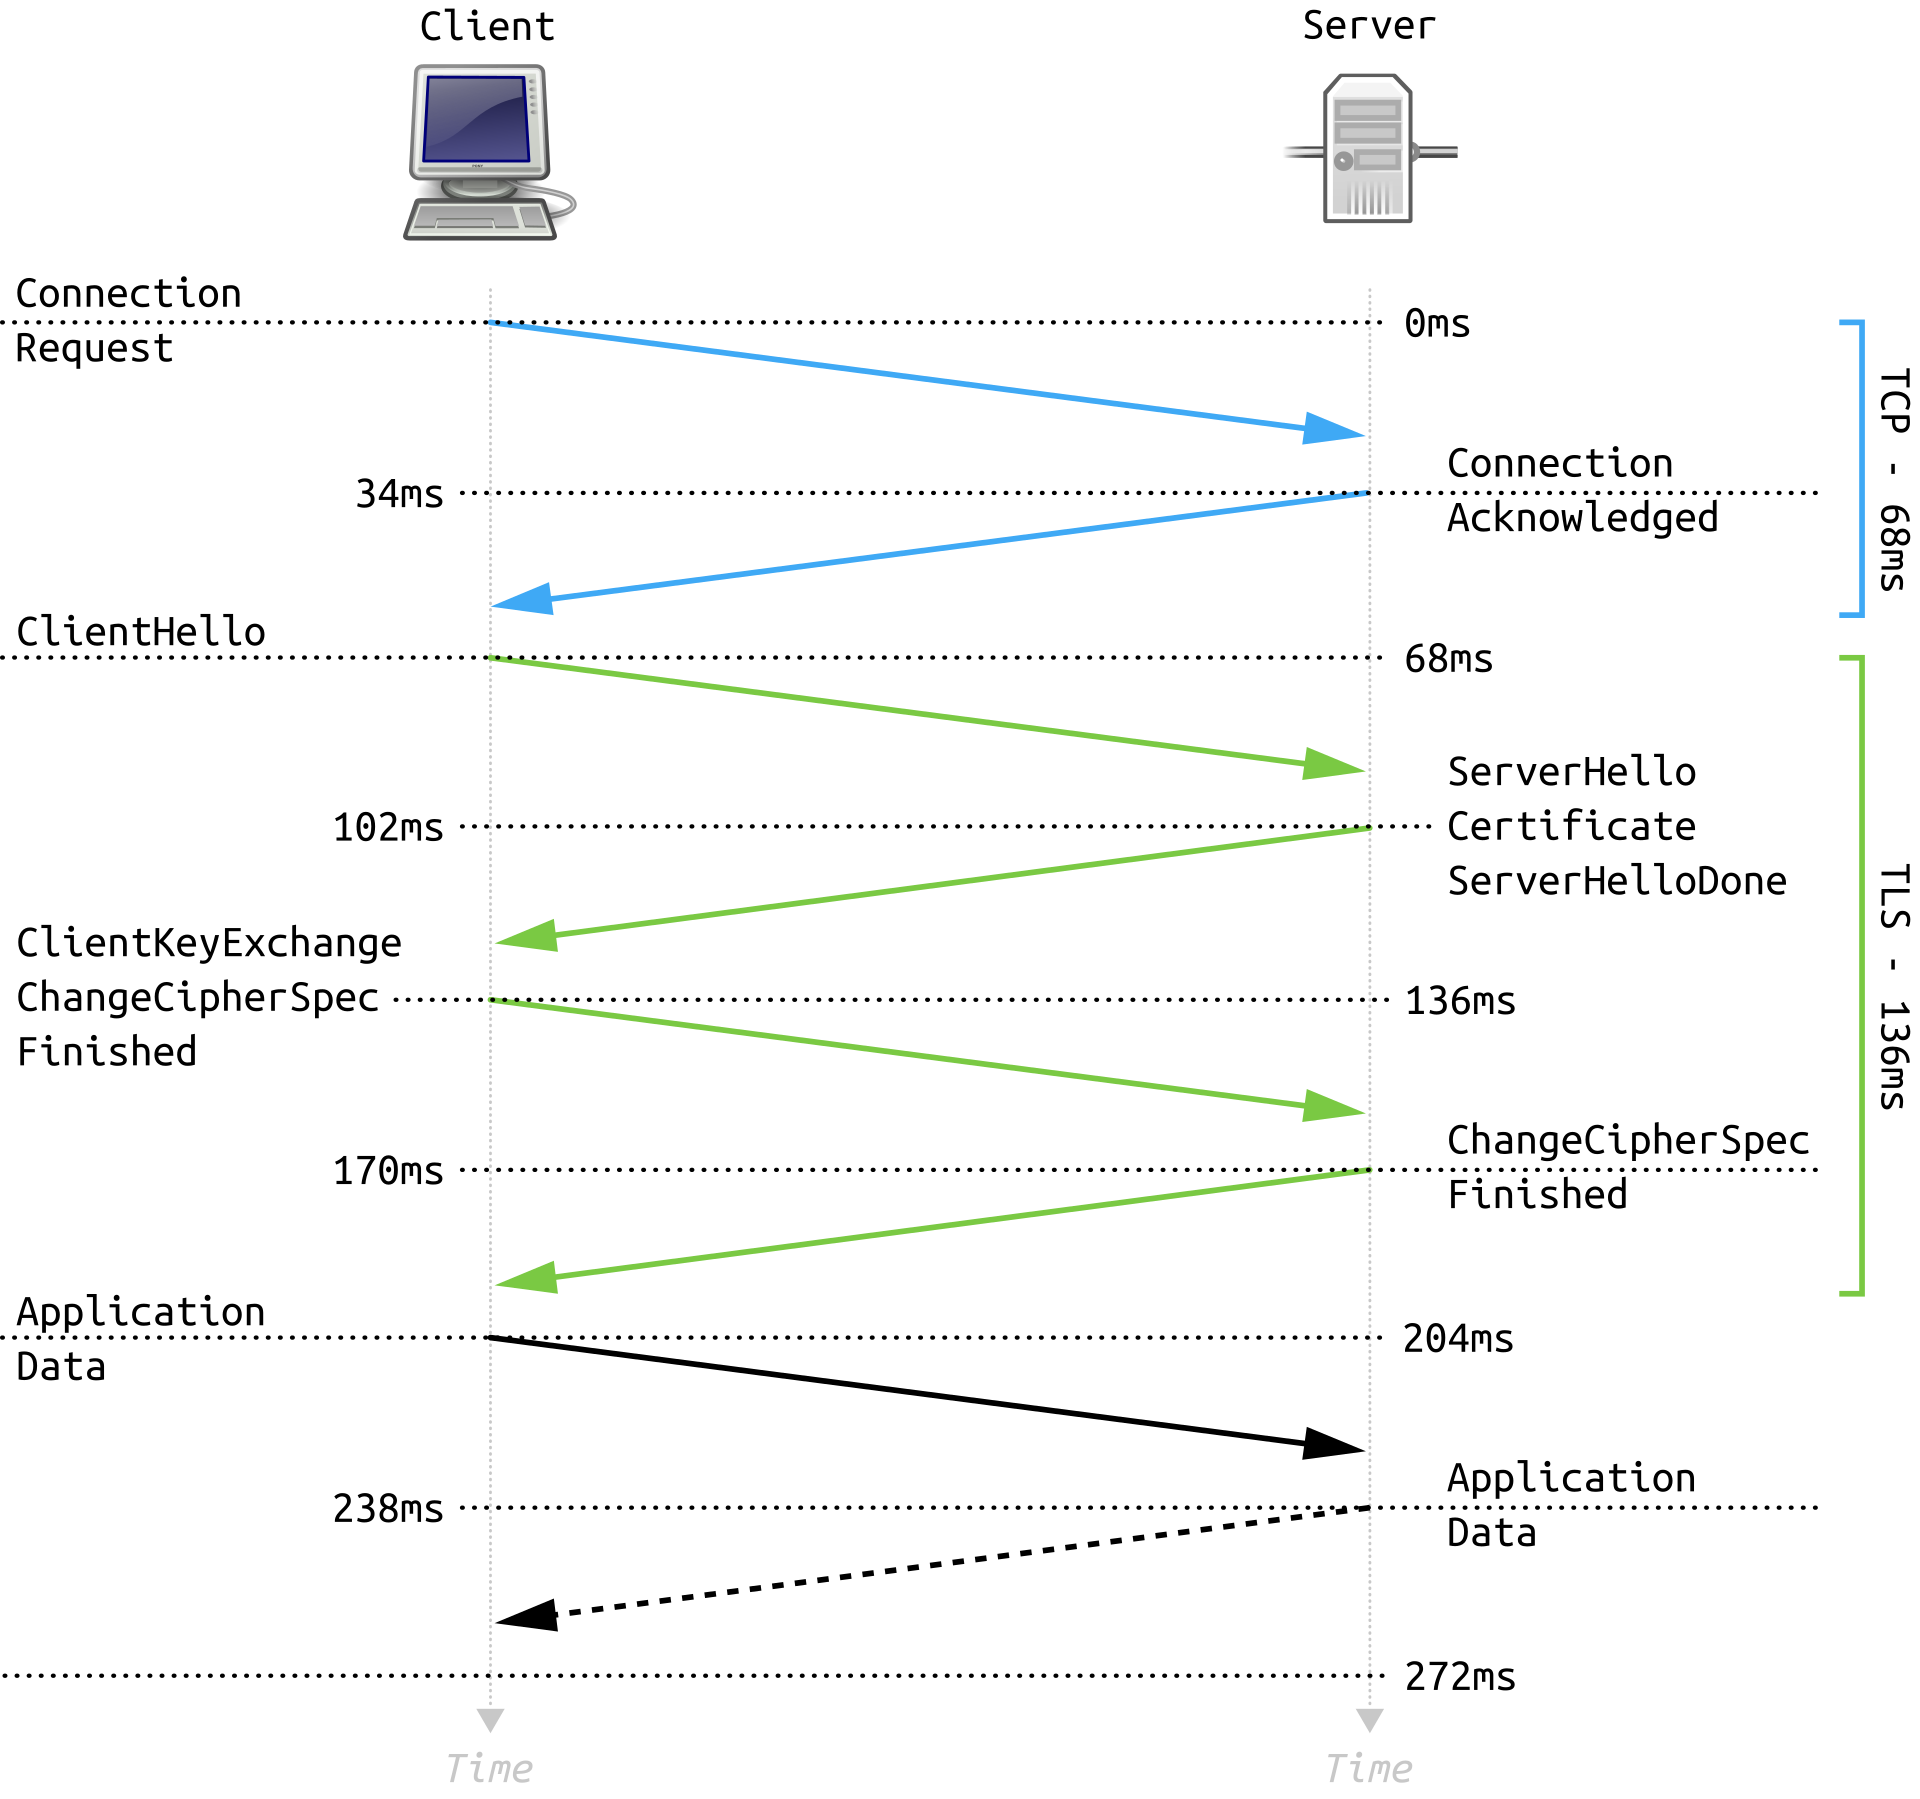
\includegraphics[width=0.8\textwidth]{Figures/Full_TLS_1_2_Handshake.png}
    \caption{TLS 1.2 Handshake}
    \label{fig:tls_handshake}
\end{figure}

The handshake can be separated into four phases:
\begin{enumerate}
    \item Negotiation: The client starts the handshake by sending a \texttt{ClientHello} message. The message contains the client's supported TLS versions, a list of supported ciphers, a random number and suggested compression methods.
    \\\\
    The server responds with a \texttt{ServerHello} message. The message contains the chosen TLS version, a chosen cipher, a random number and a chosen compression method from the supported ones the client sent before.
    \\
    The server also sends its certificate, which contains the server's public key.
    \\
    If the cipher is a version of Diffie Hellman, the server will also send a \texttt{ServerKeyExchange} message.
    \\
    The server also sends a \texttt{ServerHelloDone} message, which signals that the server is done with the negotiation phase.
    \\\\
    The client then sends a \texttt{ClientKeyExchange} message, which, depending on cipher used, contains the pre-master secret encrypted by the public key of the server, public key, or nothing.
    \\\\
    The server and client then compute a common secret, using the random numbers they shared and the pre-master secret. The common secret is also called master secret and is used to derive all other keys, like the session key or MAC key.
    
\end{enumerate}